\documentclass[border=10pt,tikz]{standalone}
\usepackage{fontspec}
\setmainfont{Apple SD Gothic Neo}
\setsansfont{Apple SD Gothic Neo}
\usepackage{tikz}
\usetikzlibrary{positioning,arrows.meta}
\begin{document}
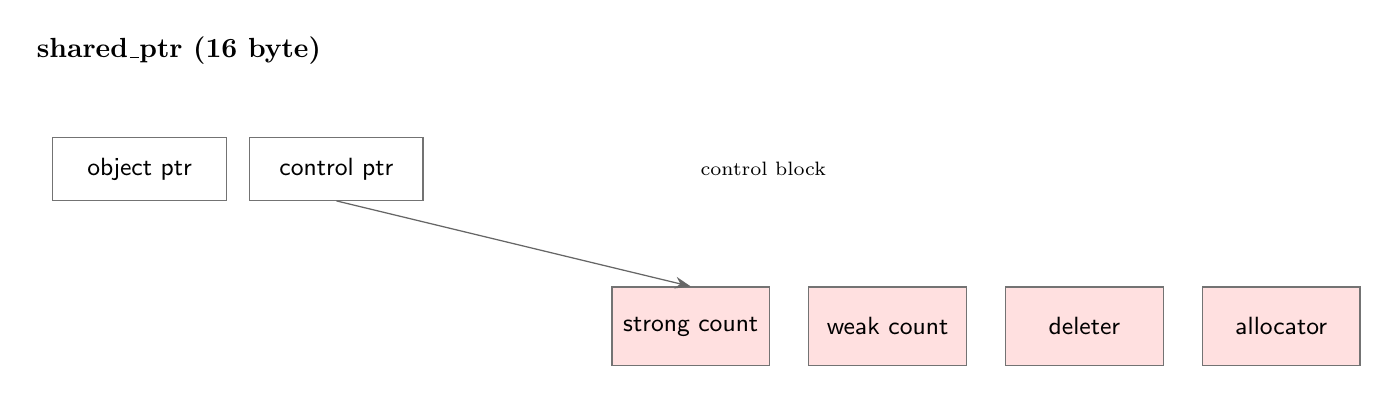
\begin{tikzpicture}[
  font=\sffamily\small,
  cell/.style={rectangle, draw=black!55, line width=0.4pt, minimum height=8mm,
               minimum width=22mm, inner sep=3pt, fill=blue!10, align=center},
  cb/.style={rectangle, draw=black!55, line width=0.4pt, minimum height=10mm,
             minimum width=20mm, inner sep=3pt, fill=red!12, align=center},
  ptr/.style={cell, fill=white},
  arr/.style={-{Stealth[length=2mm]}, draw=black!60, line width=0.45pt}
]
% sp object
\node[draw=none, fill=none, font=\bfseries] at (-5.5, 1.5) {shared\_ptr (16 byte)};
\node[ptr] (a) at (-6, 0)  {object ptr};
\node[ptr] (b) at (-3.5, 0){control ptr};

% control block
\node[cb] (sc) at (1, -2)  {strong count};
\node[cb] (wc) at (3.5,-2) {weak count};
\node[cb] (de) at (6, -2)  {deleter};
\node[cb] (al) at (8.5,-2) {allocator};

\draw[arr] (b.south) -- (sc.north);
\node[draw=none, fill=none, font=\scriptsize, anchor=west] at (1, 0) {control block};
\end{tikzpicture}
\end{document}
